\chapter{Evaluation}
\label{sec:evaluation}

\section{Methodology}

To evaluate our approach we develop and implement a number of applications
to test both the flexibility and generality of our approach but also to
ensure that we can support high-performance applications. There are in general
no standard benchmarks for FPGAs as there are for CPU/GPU systems.

\subsection{Benchmark}
\label{sec:benchmark}
Our benchmark for consists of the following applications:
\begin{itemize}
\item Numerical Differentiation
\item Black Scholes Option Pricing
\item Reverse Time Migration -- high-performance, design parallelism
\item bitonic sorting network -- a recursive design, that heavily
relies on compile-time loops, auxiliary function calls and input
groups to generate a readable description.
\end{itemize}

\subsection{Equipment}

All dataflow designs are run on Maxeler MaxWorkstation
\cite{MaxWorkstation} which comprises:
\begin{itemize}
\item Intel(R) Core(TM) i7 CPU 870 @ 2.93GHz, cache size 8192 KB
\item 16 GB DRAM
\item Vectis dataflow engine with 24 GB DRAM,
\item DFEs connect to CPU via PCI Express gen2 x8
\end{itemize}

Hardware builds usually take a long time. Additionally they are
required to meet timing and resource usage constraints. The process of
placing and routing a dataflow design can take anywhere from 20
minutes to several days. Since this is a stochastic process, usually
mutliple builds are started in parallel and when one terminates the
whole build process is terminated and that design is used. Hence the
build process requires substantial amount of DRAM and CPU cores,
particulary during the design space exploration step. Hence the builds
were ran on the Custom Computing cluster machines:

\begin{itemize}
\item \texttt{cccad3} -- 2 8 core, hyperthreaded (16 threads) Intel
  Xeon E5-2650 CPUs at 2.00GHz, 20MB cache, 189 GB DRAM
\item \texttt{cccad2} -- 2 6 core, hyperthreaded (12 threads) Intel
  Xeon X5650 CPUs at 2.67GHz, 12 MB cache, 94 GB DRAM
\item \texttt{cccad1} -- 2 6 core, hyperthreaded (12 threads) Intel Xeon
  X5650 CPUs at 2.67GHz, 12 MB cache, 118 GB DRAM
\end{itemize}

All CPU applications are compiled using GCC 4.4 with all optimisations
enabled (-O3 flag) and FPGA Designs are compiled with MaxCompiler
2012.1.

%\section{Numerical Differentiation}

%\section{Black Scholes}

\section{Reverse Time Migration}
\label{sec:RTM}
We evaluate the proposed approach by implementing a high-performance
application based on the Reverse Time Migration method for seismic
imaging which is used to detect geological structures, based on the
Earth's response to injected acoustic waves. The technique models the
propagation of injected waves using the isotropic acoustic wave
equation \cite{araya2011assessing}:
\begin{align}
\frac{d^2p(r,t)}{dt^2} + {dvv(r)}^2\bigtriangledown^2p(r,t) = f(r,t)
o\end{align}

We approximate the differential equation using stencil computation to
perform a fifth-order Taylor expansion in space and first-order Taylor
expansion in time.

We use \FAST{} to implement the dataflow kernels and aspects to
generate multiple configurations for the design by creating two
kernels that are used to control the memory command read and write
streams (CmdRead, CmdWrite) and the computation kernel (RTM).

To illustrate the potential benefits of our approach we analyse the
results of using the debugging aspect of Section
\ref{sect:asp_debug}. Table~\ref{table:loc} compares the number of
lines of code required for the \FAST{} with aspect design with the
equivalent MaxCompiler implementation showing a reduction in code size
of up to 42\% for the run-time reconfigurable design and a reduction
in the number of API calls (including debug calls) of up to 67\% which
translate to increased productivity.

\begin{table}[!h]
  \renewcommand{\arraystretch}{1.2}
  \centering
  \caption{Code measures for the RTM kernels comparing \FAST{} and
    MaxCompiler.}
  \label{table:loc}
  \begin{tabular}{c|ccc|cc}
    \hline
    \multirow{2}{*}{\bf{Kernel}} & \bf{Aspect } & \multicolumn{2}{c|}{\bf{\FAST{}}} & \multicolumn{2}{c}{\bf{MaxCompiler}}                   \\
    \                            & \bf{LOC}     & \bf{LOC}                       & \bf{\# API calls} & \bf{LOC} & \bf{\#API Calls} \\
    \hline \hline
    CmdRead                      & 12           & 26                             &      6         & 59       &      39        \\
    CmdWrite                     & 12           & 28                             &      39        & 79      &       56         \\
    RTM Static                   & 12           & 246                            &     43         & 403     &       175        \\
    RTM RTR                      & 12           & 377                            &     91         & 669     &       275       \\
  \end{tabular}
\end{table}

\subsection{Results}

Results of the design space exploration using the aspect in
Fig.~\ref{fig:aspect-exploration} with variable mantissa illustrate
the trade-offs between accuracy and resource usage
(Fig.~\ref{fig:precision}). We observe irregular, large variations
when decreasing the mantissa from 18 to 16 and 24 to 22 which is the
effect of the backend tools mapping arithmetic to a combination of
both DSPs and LUT/FF elements. The mantissa boundaries at which this
optimisation occurs are platform specific, depending on the
architecture of the DSPs. Hence, automating this optimisation via
aspects and decoupling it from the original source code makes the
application more portable and facilitates discovery of interesting
trade-off opportunities using design space exploration.

\begin{figure}[!h]
\centering
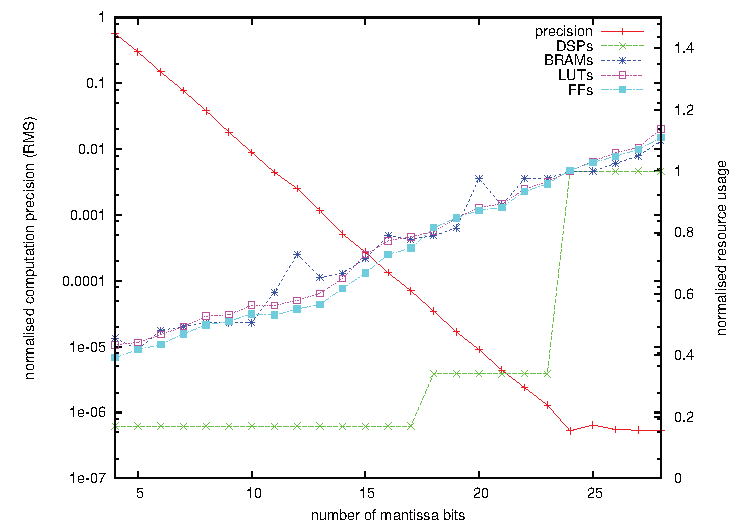
\includegraphics[scale=1.2]{figs/pre}
\caption{Exploration of accuracy vs resource usage trade-offs using the aspect
shown in Fig.~\ref{fig:aspect-exploration} with variable mantissa.}
\label{fig:precision}
\end{figure}

The DSP balancing aspect shown in Fig.~\ref{fig:aspect-DSP} allows to
explore the resource trade-offs of implementing arithmetic operations
in either DSPs or LUTs and FFs (Fig.~\ref{fig:arith}) and helps to
avoid over mapping on DSPs for arithmetic intensive applications.

\begin{figure}[!h]
\centering
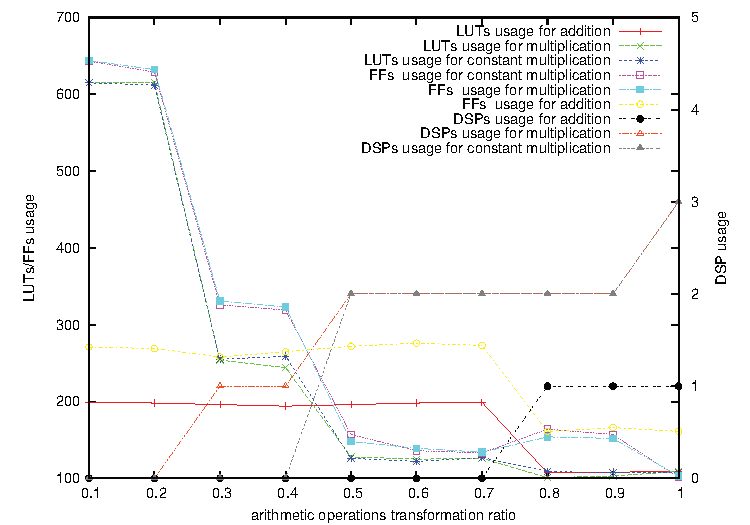
\includegraphics[scale=1.2]{figs/arith}
\caption{Exploration of DSP and LUT/FF balancing for functional units
  implementing a single arithmetic operation using the aspect shown
  in Fig.~\ref{fig:aspect-DSP}.}
\label{fig:arith}
\end{figure}

Design space exploration using the aspect in
Fig.~\ref{fig:aspect-exploration} with increasing parallelism level
can be used to investigate design scalability. For example, for the
described RTM implementation, Fig.~\ref{fig:scalability} shows that
performance scales linearly with the number of parallel pipelines and
that significant speedups can be obtained by the \FAST{} dataflow
design compared to the CPU only implementation. Depending on the
problem size, our approach can be used to achieve a significant
speedup over software only versions which is comparable with the best
published FPGA results for static designs
\cite{Xinyu:Qiwei:Luk:Qiang:Pell:2012}, \cite{araya2011assessing}.


\pgfplotsset{every axis x label/.style={
  at={(0.5,0)},
  below,
  yshift=-5pt}}

\pgfplotsset{every axis y label/.style={
  at={(0,0.5)},
  xshift=-20pt,
  rotate=90}}


\begin{figure}[!h]
  \centering
  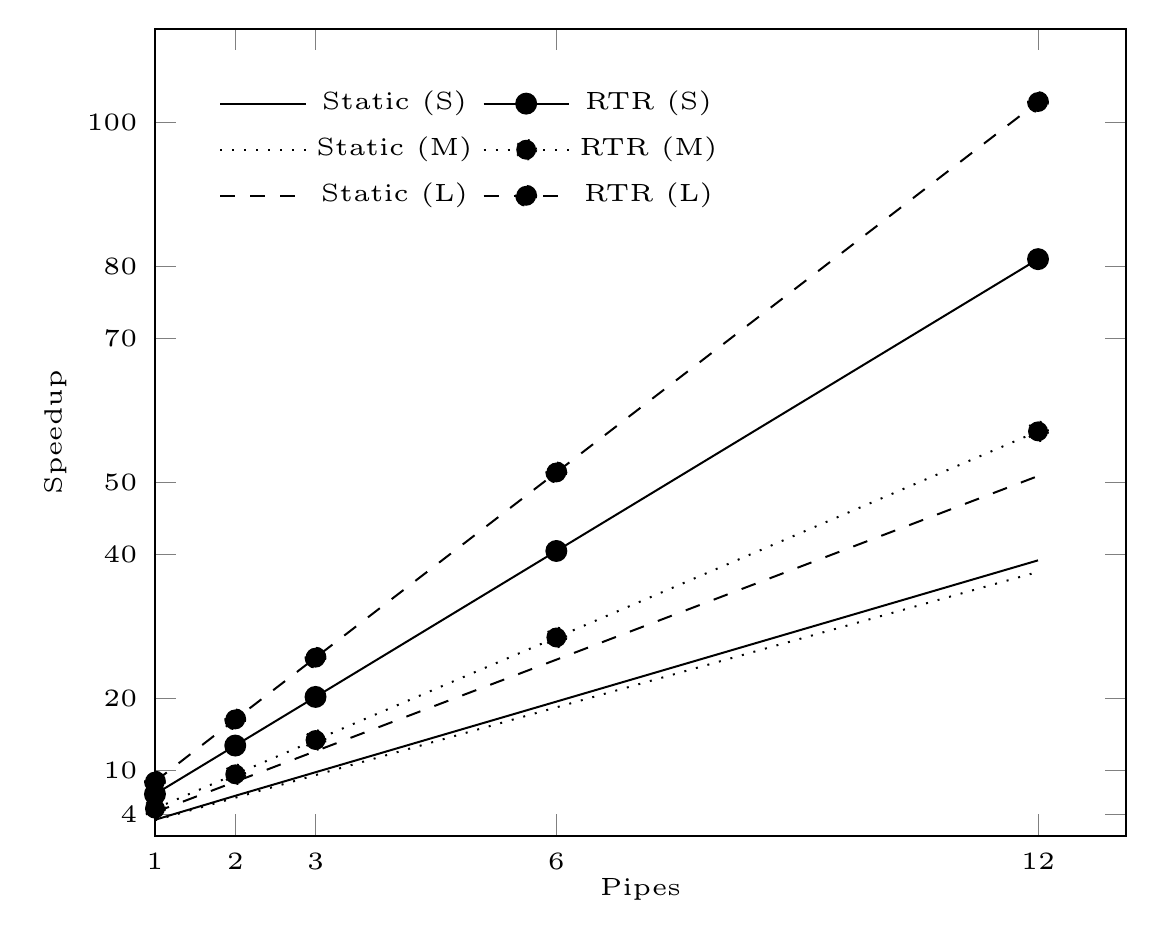
\begin{tikzpicture}[scale=1.8]
    \selectcolormodel{gray}
    \begin{axis}[
        xmin=1,
        ymin=1,
        %no markers,
        font=\tiny,
        xlabel=Pipes,
        ylabel=Speedup,
        xtick={1,2,3,6,12},
        ytick={4, 10, 20, 40, 50, 70, 80, 100},
        legend columns=2,
        legend entries={
          Static (S),
          RTR (S),
          Static (M),
          RTR (M),
          Static (L),
          RTR (L)},
        legend style={
          draw=none,
          at={(0.05,0.85) },
          anchor=west
        }
      ]

      \addplot[mark=none] coordinates {
        (1, 3.2)
        (2, 6.53)
        (3, 9.8)
        (6, 19.6)
        (12, 39.2)
      };
      \addplot[mark=*] coordinates {
        (1, 6.75)
        (2, 13.5)
        (3, 20.25)
        (6, 40.5)
        (12, 81)
      };
      \addplot[dotted] coordinates {
        (1, 3.13)
        (2, 6.26)
        (3, 9.4)
        (6, 18.8)
        (12, 37.6)
      };
      \addplot[mark=*, dotted] coordinates {
        (1, 4.75)
        (2, 9.51)
        (3, 14.27)
        (6, 28.5)
        (12, 57.1)
      };
      \addplot[mark=none, dashed] coordinates {
        (1, 4.25)
        (2, 8.48)
        (3, 12.725)
        (6, 25.42)
        (12, 50.9)
      };
      \addplot[mark=*, dashed] coordinates {
        (1, 8.5)
        (2, 17.13)
        (3, 25.7)
        (6, 51.4)
        (12, 102.8)
      };
    \end{axis}
  \end{tikzpicture}
  \caption{Scalability of the RTM dataflow design explored using the aspect
shown in Fig.~\ref{fig:aspect-exploration}.}
  \label{fig:scalability}
\end{figure}



Fig.~\ref{fig:scalability} also shows a model of the performance
benefits of using a run-time reconfigurable implementation generated
using the proposed aspect-oriented approach. Two configurations were
created for the RTM \FAST{} kernel. Since, in our model, during the
first half of the execution time, the backward propagation and imaging
functions are idle, the first configuration requires only half the
resources. Hence, the number of parallel pipelines can be doubled,
halving the execution time of the first configuration. The speedup
obtained is comparable to \cite{Xinyu:Qiwei:Luk:Qiang:Pell:2012}, but
the partitioning and optimisation exploration process is automated via
aspects, which increases developer productivity. The automated process
improves portability of the design, allowing optimisations based on
design space exploration to be carried out on various platforms (hence
subject to varying resource constraints) without manual intervention.


\begin{sidewaystable}
  \begin{tabularx}{\textwidth}{p{3.5cm}|X|X|X|X|X|X|X|X|X|X|X|X|X|}
    Aspects & DSP Balance & Par & Mem Freq & Width & FPGA  Time (Ms) & Total Time (s) & Total Power (Watt) & Dyn. Power (Watt) & LUT (\%) & FF(\%) & BRAM (\%) & DSP (\%) & Build Time \\
    \hline \hline
    \multirow{5}{2cm}{OptimizeDSPUsage, ExploreParallelism}     & Bal.    & 1   & 303      & 8\_24 & 492             & 3.347          & 117                & 30                & 19.89    & 14.13  & 23.31     & 1.69     & 1h 49      \\
            & None        &     &          &       & 492             & 3.453          & 117                & 30                & 22.62    & 15.56  & 23.31     & 0        & 2 h 9      \\
            & Full        &     &          &       & 492             & 3.103          & 117                & 30                & 17.68    & 12.79  & 23.31     & 5.8      & 2 h 2      \\
            \hline
            & Bal.    & 2   &          &       & 247             & 2.917          &	121                & 34                & 25.44    & 25.44  & 24.53     & 3.37     & 2h30       \\
            & None        &     &          &       & 247             & 3.006          &	121                & 34                & 30.95    & 20.53  & 24.53     & 0        & 3h5        \\
            & Full        &     &          &       & 246             & 3.153          &	121                & 34                & 21.18    & 15     & 24.44     & 11.61    & 2h8        \\
            \hline
            & Bal.    & 3   &          &       & 225             & 3.506          & 121                & 34                & 31.56    & 21.32  & 24.06     & 5.06     & 2h30       \\
            & None        &     &          &       & 224             & 3.124          & 121                & 34                & 39.16    & 25.61  & 24.06     & 0        & 3h20       \\
            & Full        &     &          &       & 226             & 3.123          & 125                & 38                & 25.06    & 17.3   & 23.97     & 17.41    & 2h18       \\
            \hline
            & Bal.    & 6   &          &       & 226             & 3.125          & 125                & 38                & 52.61    & 30.52  & 20.12     & 17.41    & 3h17       \\
            & None        &     &          &       & 223             & 3.156          & 125                & 38                & 65.11    & 40.58  & 28.95     & 0        & 4h50       \\
            & Full        &     &          &       & 224             & 3.016          &	122                & 35                & 35.63    & 24.11  & 27.73     & 34.82    & 3h42       \\
            \hline
    \multirow{5}{2cm}{OptimizeWordWidth, OptimizeFrequency, ExploreParallelism}        & Full        & 6   & 303      & 8\_22 & 224             & 2.98           & 122                & 35                & 45.02    & 31.17  & 27.73     & 15.18    & 3h13       \\
            &             &     &          & 8\_20 & 224             & 3.006          &	122                & 35                & 43.54    & 29.96  & 27.16     & 15.18    & 3h30       \\
            &             &     &          & 8\_18 & 224             & 3.076          & 122                & 35                & 40.81    & 28.68  & 26.88     & 15.18    & 3h13       \\
            &             &     &          & 8\_16 & 224             & 3.033          & 122                & 35                & 39.62    & 26.44  & 26.6      & 10.12    & 2h50       \\
            &             &     &          & 8\_24 & 82              & 1.723          & 122                & 35                & 34.13    & 24.09  & 27.73     & 34.82    & 4h17       \\
            \hline
            &             & 2   & 400      & 8\_24 & 247             & 3.133          &	122                & 35                & 21.32    & 14.98  & 24.44     & 11.61    & 2h30       \\
            &             & 3   &          & 8\_24 & 164             & 2.964          & 122                & 35                & 25.43    & 17.28  & 23.97     & 17.41    & 2h35       \\

  \end{tabularx}
\end{sidewaystable}


\section{Bitonic Sort}

We implement a design for sorting $n$ arrays of size $k = (4, 8, 32,
64, 128, 256)$ elements. We compare the performance of the design with
the ANSI C implementation of \texttt{qsort()} which is a hybrid of
insertion-sort and quicksort. For a fixed network size, we vary the
input size to compare the software and hardware implementations and
report the average results of 50 runs.



1. Bitonic sort
\begin{enumerate}
\item $complexity = network depth = n(logn)/2 =  (O(log^2(n)))  $
\item $ comparators = n (logn) (logn + 1) / 4 = O(nlog^2(n)) $
\end{enumerate}


2. The software algorithm is qsort (<stdlib.h>
http://www.umcs.maine.edu/~chaw/200801/capstone/n/qsort.c). This is a
hybrid quick sort - insertion sort.


\subsection{HW/SW Performance comparison}

The results show that the hardware version outperforms the software
version for values of n larger than $2^4$ with speedups increasing from
1.25X to 24X, in proportion with the value of n.  Also the execution
time is dominated by data transfer time over PCIe from main memory to
the FPGA accelerator. The impact of the pipeline stages is so small
(less that 1%) that it cannot be measured accurately using the Linux
timing utilities ( gettimeofday() ).

\subsection{Reconfiguration Cutpoint}

Given that execution time is dominated by the transfer time,
reconfiguring the design to increase parallelism will bring a small
performance benefit.  The situation changes when the network is used
as part of a general purpose sorting algorithm. The complexity $( O(N/k
* logn * log(n/k)) $ decreases linearly with the increase in the network
width. This would provide the motivation to adapt the network to input
patterns, switching to larger networks for small observed values.

Hence it is only necessary to reconfigure when a change in the input
pattern is detected that requires us to use a different
precision. (e.g. floating point vs int).

One factor to consider is that, reducing to smaller network sizes can
also decrease the communication overhead. Since all network inputs
must be present, additional padding is required for arrays that are
not of a length which is a power of two. (Requires additional data)


\subsection{Word Length}

Results of varying the word length show that decreasing word width and
varying the type (floating or fixed point, based on the input
characteristics) allow us to build larger network sizes. This can more
than double the performance of networks for small input values.

\subsection{Results}

\begin{table}[!ht]
  \begin{tabularx}{\textwidth}{X | X | X | X | X | X}
    \hline
    Type & Width & Max. Network Size & Resource Usage (LUT/FF) & Overmaps At Next Size & Meets Timing at Next Size \\
    \hline
    \hline
    int & 32 & 128 & 127344 / 260434 & yes & no \\
    \hline
    int & 16 & 128 & 127344 / 260434 & no (23343 / 343332) & no \\
    \hline
    int & 8 & 256 & 95430 / 188245 & no (260878 / 458532) & no \\
    \hline
    float & 32(8, 24) & 64 & 101758 / 107901 & yes & no \\
    \hline
    fixed point & (8, 24) & 128 & 127344 / 260434 & yes & no \\
    \hline
    fixed point & (24, 8) & 128 & 127344 / 260434 & yes & no \\
  \end{tabularx}
  \caption{Results of exploring different network sizes and data types for the bitonic sorting network}
\end{table}

\begin{table}
  \begin{tabularx}{\textwidth}{X|X|X|X|X|X|X}
    \hline
    Network Size        & log(n)      & CPU Time & FPGA Time & Compute Speedup & FPGA Total Time & FPGA Total Speedup \\
    \hline \hline
\multirow{10}{*}{128}   & 14          & 0.156162 & 0.006564  & 23.79           & 1.006564        & 0.1551             \\
                        & 15          & 0.312428 & 0.013028  & 23.98           & 1.013028        & 0.3084             \\
                        & 16          & 0.624328 & 0.026263  & 23.77           & 1.026263        & 0.6084             \\
                        & \textbf{7}  & 1.24981  & 0.051905  & 24.08           & 1.051905        & \textbf{1.1881}    \\
                        & 18          & 2.49068  & 0.102083  & 24.4            & 1.102083        & 2.26               \\
                        & 19          & 4.98994  & 0.199928  & 24.96           & 1.199928        & 4.1585             \\
                        & 20          & 9.97521  & 0.400709  & 24.89           & 1.400709        & 7.1215             \\
                        & 21          & 19.9636  & 0.807231  & 24.73           & 1.807231        & 11.0465            \\
                        & 22          & 39.9202  & 1.614437  & 24.73           & 2.614437        & 15.2691            \\
                        & 23          & 79.8726  & 3.203924  & 24.93           & 4.203924        & 18.9995            \\
    \hline
    \multirow{8}{*}{64} & 16          & 0.271163 & 0.012983  & 20.89           & 1.012983        & 0.2677             \\
                        & 17          & 0.541016 & 0.025841  & 20.94           & 1.025841        & 0.5274             \\
                        & \textbf{18} & 1.08533  & 0.052019  & 20.86           & 1.052019        & \textbf{1.0317}    \\
                        & 19          & 2.16697  & 0.10265   & 21.11           & 1.10265         & 1.9652             \\
                        & 20          & 4.33626  & 0.203208  & 21.34           & 1.203208        & 3.6039             \\
                        & 21          & 8.66081  & 0.406241  & 21.32           & 1.406241        & 6.1588             \\
                        & 22          & 17.3281  & 0.806145  & 21.5            & 1.806145        & 9.594              \\
                        & 23          & 34.6705  & 1.617021  & 21.44           & 2.617021        & 13.2481            \\
    \hline
\multirow{6}{*}{32}     & 18          & 0.458403 & 0.026085  & 17.57           & 1.026085        & 0.4467             \\
                        & 19          & 0.917055 & 0.051485  & 17.81           & 1.051485        & 0.8722             \\
                        & \textbf{20} & 1.83439  & 0.100844  & 18.19           & 1.100844        & \textbf{1.6663}    \\
                        & 21          & 3.67453  & 0.203696  & 18.04           & 1.203696        & 3.0527             \\
                        & 22          & 7.35396  & 0.404244  & 18.19           & 1.404244        & 5.237              \\
                        & 23          & 14.6802  & 0.810293  & 18.12           & 1.810293        & 8.1093             \\
\hline
   \multirow{5}{*}{16}  & 19          & 0.375978 & 0.026123  & 14.39           & 1.026123        & 0.3664             \\
                        & 20          & 0.759506 & 0.051846  & 14.65           & 1.051846        & 0.7221             \\
                        & \textbf{21} & 1.49907  & 0.102618  & 14.61           & 1.102618        & \textbf{1.3596}    \\
                        & 22          & 3.00802  & 0.201457  & 14.93           & 1.201457        & 2.5036             \\
                        & 23          & 5.99392  & 0.406334  & 14.75           & 1.406334        & 4.2621             \\
  \end{tabularx}
  \caption{Speedup results for the FPGA sorting network compared to
    the CPU only version. Points after which it becomes convenient to
    use FPGA acceleration are highlighted.}
\end{table}


\begin{comment}
\begin{figure}[!h]
  \centering
  \vspace{0.35cm}
  \hspace{-8mm}
  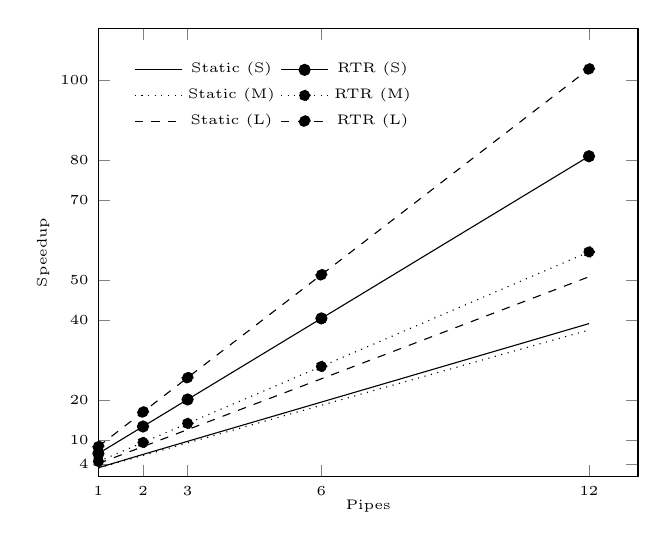
\begin{tikzpicture}[scale=1]
    \selectcolormodel{gray}
    \begin{axis}[
        xmin=1,
        ymin=1,
        %no markers,
        font=\tiny,
        xlabel=Pipes,
        ylabel=Speedup,
        xtick={1,2,3,6,12},
        ytick={4, 10, 20, 40, 50, 70, 80, 100},
        legend columns=2,
        legend entries={
          Static (S),
          RTR (S),
          Static (M),
          RTR (M),
          Static (L),
          RTR (L)},
        legend style={
          draw=none,
          at={(0.05,0.85) },
          anchor=west
        }
      ]

      \addplot[mark=none] coordinates {
        (1, 3.2)
        (2, 6.53)
        (3, 9.8)
        (6, 19.6)
        (12, 39.2)
      };
      \addplot[mark=*] coordinates {
        (1, 6.75)
        (2, 13.5)
        (3, 20.25)
        (6, 40.5)
        (12, 81)
      };
      \addplot[dotted] coordinates {
        (1, 3.13)
        (2, 6.26)
        (3, 9.4)
        (6, 18.8)
        (12, 37.6)
      };
      \addplot[mark=*, dotted] coordinates {
        (1, 4.75)
        (2, 9.51)
        (3, 14.27)
        (6, 28.5)
        (12, 57.1)
      };
      \addplot[mark=none, dashed] coordinates {
        (1, 4.25)
        (2, 8.48)
        (3, 12.725)
        (6, 25.42)
        (12, 50.9)
      };
      \addplot[mark=*, dashed] coordinates {
        (1, 8.5)
        (2, 17.13)
        (3, 25.7)
        (6, 51.4)
        (12, 102.8)
      };
    \end{axis}
  \end{tikzpicture}
  \caption{Scalability of the RTM dataflow design explored using the aspect
shown in Fig.~\ref{fig:aspect-exploration}.}
  \label{fig:scalability}
\end{figure}
\end{comment}
